\chapter{Flexibility between various datasets}

To build a Deep Learning system that works for some data, it needs to learn how to process them. To do that, we have to make it learn correct weights (for each of its layers) by doing supervised learning with a given dataset. But the characteristics of the dataset will obviously have a huge influence on the learning, so we have to be careful while choosing and/or building the dataset. We also will see how to deal efficiently with different dataset with one single DL system. In this section, we will focus ourselves on datasets composed of pictures, but we have to keep in mind that we also can work with other kind of data.



\section{A wide range of datasets}
\subsection{Many characteristics}
It exists many datasets for computer vision, and they all differ by some given characteristics :
\begin{itemize}
\item Their context : A dataset can be done with many different contexts, or with only a specific one. Indeed, it can be built with multiple kind of pictures : indoor, outdoor, by night, aerial, alone-object focus... A dataset with multiple kind of pictures is more difficult to learn by the system because it would involve to learn a lot of features for a lot of different objects and to understand that each of them can also have multiple instances (by night, reverse, half-hidden, ...). On the other hand, if we have a dataset composed in integrity by cat pictures, the system will learn something really specific (cat recognition) and won't be flexible to other images.
\item Their number of classes : Most of the pictures of our dataset would represent several objects and not only one defined object. Indeed, even a simple cat picture would have a complex background (plant, ground, wall, kennel, ...) and we have to define if we want to extract some information on this. Most of the datasets have a small number of classes but the biggest ones can grew up to few thousands classes.
\item Their way to segment the pictures : the way to segment the image is different, it depends on the future application of the system. For example, if we want to build a system able to distinguish pictures of cats and dogs, we won't need to segment them, a simple label corresponding to the appropriate class attached to the picture would be enough. If we also want to locate the pet, we should then attach the label with the location. The table~\ref{fig:part2:segmentation_comparison} shows three examples of segmentation, including pixel-wise labelling.

\begin{figure}[ht!]
  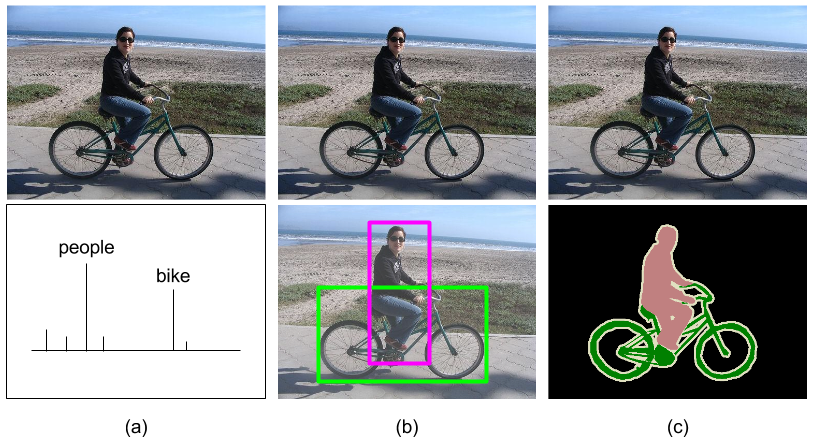
\includegraphics[width=\linewidth,center]{images/part2/segmentation_comparison.png}
  \caption{Different segmentation kind}\textbf{
  \label{fig:part2:segmentation_comparison}}
\end{figure}

\end{itemize}


\subsection{A quick state of the art} \label{2:datasets:soa}
Basically, few dataset are famous in computer vision, here is a non-exhaustive list of them, and a visual example for each of them is also provided as appendix~\ref{fig:appendices:datasets_comparison} :
\subsubsection{MNIST} This database contains 70.000 handwritten digits which have been size-normalized and centered in a fixed-size image. The works of Yann LeCun~\cite{LECU95, LECU98}, one of the father of Deep Learning, are based on this dataset and allowed a system to convert a written text into a typing text. Each image has a single label, corresponding to its appropriate letter or number.
\subsubsection{ImageNet} One of the biggest dataset currently used for Deep Learning system, it is composed by more than 14 million images, representing situations in the world without limitation (group of people, table, dog in kennel, candy shop, ...). These images are labelled according to more than 21 thousand classes, divided into 27 high level categories (fruit, person, vehicle, ...). Every single image have one label, corresponding to the class of the main object in the picture, and about one million of them also have a bounding box annotations (the objects in the images are bounded by a square). Most of the architectures are tested on ImageNet because of its size, and it finally turns into a really famous challenge (ILSVRC Challenge~\cite{RUSS15}).
\subsubsection{Pascal VOC} An other famous image dataset, pretty similar to ImageNet by its diversity, is the Pasxal VOC's. The main difference is the labelling methods : Pascal VOC proposes a semantic segmentation of its images, where each pixel of each label is labelled as belonging to one class. The other main difference is, obviously, its size (it is much longer to segment an image than simply label it), so Pascal VOC 2012 has almost 12 thousand images segmenting 21 different classes. Also, the images don't respect any size normalization. This dataset is the most famous in the semantic segmentation field, and also have its own challenge~\cite{EVER10}.
\subsubsection{SBD} The Berkeley Segmentation Dataset~\cite{MART01} is similar to Pascal VOC and ImageNet by the diversity of its images. It is composed of 12 thousand images which all have a boundary segmentation. This kind of segmentation can be used for pixel wise labelling, improving the accuracy of the boundaries.
\subsubsection{MS COCO} This dataset, from Microsoft~\cite{LIN14}, is less famous than the previous ones, but also provides a large dataset with partial semantic segmentation (for each image, the labelling contains at most 10 instance per given categories). For images containing a highest number of instances (such as crowds for people, car parks for cars, forests for trees, ...) areas are notated as "crowd". The dataset is large, composed of 300.000 images, which are divided in 80 different categories.
\subsubsection{CamVid} The CamVid dataset~\cite{BROS09} is not famous at all in the Deep Learning field, but we cite it here because it is, in a way, really close to the dataset we are going to create with aerial-views. Indeed, it is composed by images captured from the perspective of a driving automobile. All of them have a complete semantic segmentation, and the background class ("unknown" class) has a really small place in the dataset. This dataset is composed of over 700 images, divided in 32 semantic high level classes, covering most of a driving-based view.


\section{Focus on aerial views}
\subsection{Many questions to answer}
As we saw previously, we have to answer to many questions while creating a dataset. Here is a list of few of them, focusing on the aerial views problem.

First, we have to define the context. In the case of this project, we want some aerial-views, so all the images are going to be taken from the perspective of a drone. Few questions still remain there, like the height of the drone, because the shape of objects drastically changes with the point of view. Also, we have to wonder about the angle of the camera : it can be oriented to the ground, or a bit elevated (oblique view). Finally, it is also important to decide where does the drone will fly. Indeed, if it flies only above fields, our system would not be able to segment buildings, because he would see them for the first time. Of course, a single dataset can merge few of these characteristics (such as views from 50m and 70m), but it may affect the learning if the dataset is too small.

Secondly, the labelling type is important, but also quite obvious for this project. The aim of the project is to offer a detailed information of its visual environment to the drone in real time, so we want the most-detailed level of information. The pixel-wise segmentation (defining one single class per pixel) is a good way to build this information. We also saw the example of SBD in section~\ref{2:datasets:soa} that only labels boundaries for each image. It also can be interesting for our project, but the efficiency of this kind of segmentation has not been proven yet and it is simple to generate this boundary from the pixel-wise segmentation (the reciprocal is not true).

Thirdly, and maybe one of the most important point, we have to define the number of classes. Most of aerial views would display some common objects, such as building, pedestrians, cars, pavements... but also some uncommon objects like train tracks, trucks, sport areas... A solution is to analyse each image of our dataset before doing segmentation, to note every single objects present in it, and to deduce the final number of classes. The problem is that it would involve a too large number of classes with some of them really rare, and it may disturbs the learning. An other solution is to resume all of these classes into few big categories (pavement, road, car parks all labelled as "paved ground" for example), but it also should depend on the final application of the system : do we need to distinguish car parks ? Or recognizing it as a paved ground is enough ?

Fourthly, the precision of the dataset. Indeed, what would be the size of the image, and the level of detail ? If we saw a pedestrian on a few amount of pixel, should we consider him ? Moreover, the size of the image should respect the computation constraints of the GPU (it also depends on the memory required by the architecture) and we should also take in consideration the real-time notion.

Fifthly, the size of the dataset. A biggest dataset would offer a better accuracy and flexibility if its diversity increases with its size. But building a big dataset takes a long time, and involved the work of many people~\cite{LIN14}, so we have to determine what can be the most interesting alternative.


\subsection{What we chose to do}
We chose to build two different small datasets. Indeed, it is more interesting to run our experiments on two different sets for testing the reproducibility of them, and also to play with our architectures on both of them, to see how it affects the learning. For both datasets, we chose to use the same general classes.
\begin{enumerate}
\item The first dataset is taken from the swiss company senseFly\footnote{sensefly.com/drones/example-datasets} database. We used the dataset \textit{senseFly HGsite} and did pixel-wise segmentation on 100 images. On this dataset, the drone only flies above one area with industrial areas, fields, and residential districts. Each image has a size of 4608x3456, is taken at 88m of altitude, and has a view pointing to the ground (90 degrees).
\item The second dataset has been done by our own drone, in Okutama (Japan), and the images are taken from two different areas : around a baseball field and around a highschool. These two areas present some industrial, residential, sport areas and some forests. Each of the 28 images has a size of 3840x2160, is taken at 90m of altitude, and has, as above, a view pointing to the ground (90 degrees).
\end{enumerate}
For both of them, we chose to segment the following 10 classes : background, structures, building, pavement, non-paved ground, train tracks, plants, vehicles, water and people. The figure~\ref{fig:datasets_example} shows an example of this two datasets.

\begin{figure}[ht!]
\centering
\begin{subfigure}{.5\textwidth}
  \centering
  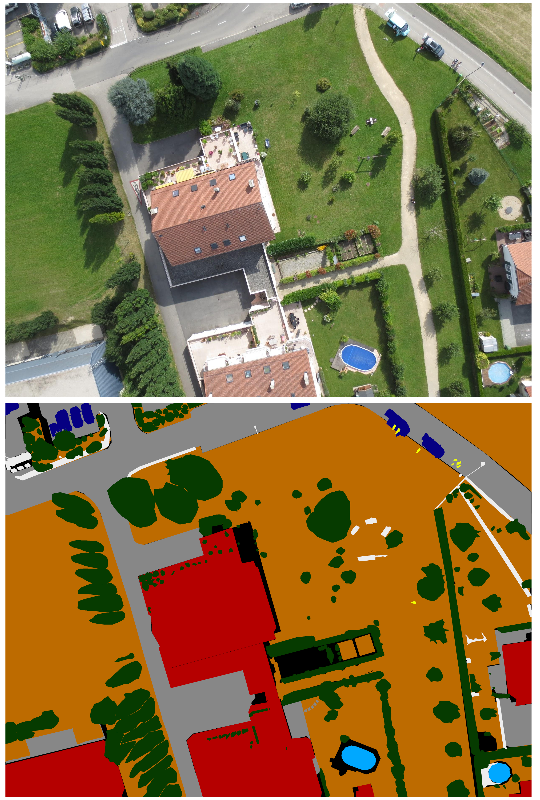
\includegraphics[height=7cm]{images/part2/swiss_example.png}
  \caption{Swiss dataset}
  \label{fig:part2:swiss_example}
\end{subfigure}%
\begin{subfigure}{.5\textwidth}
  \centering
  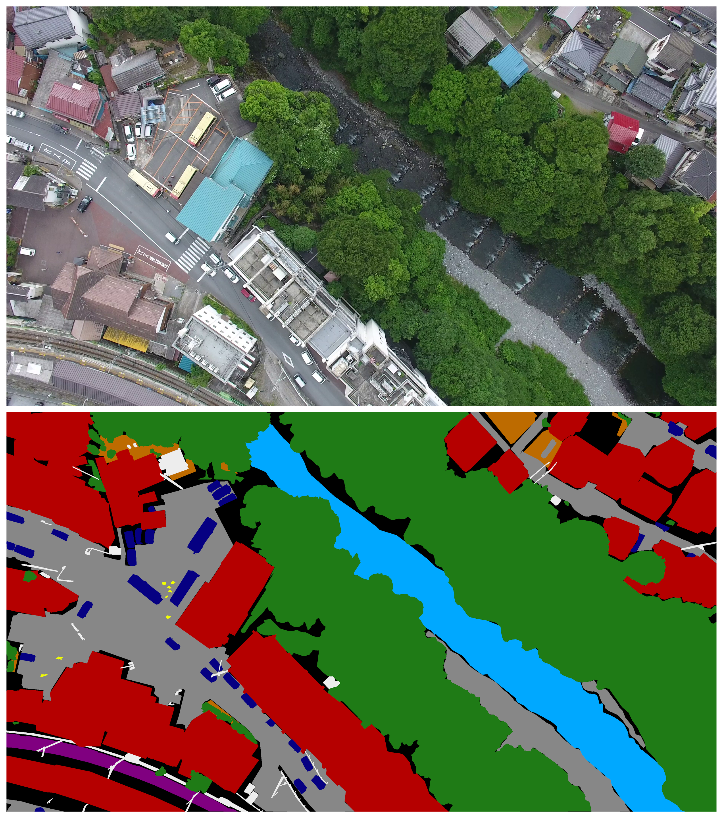
\includegraphics[height=7cm]{images/part2/oku_example.png}
  \caption{Okutama dataset}
  \label{fig:part2:oku_example}
\end{subfigure}
\caption{Datasets created}
\label{fig:datasets_example}
\end{figure}



\section{Deep Transfer Learning}
\subsection{Why do we have to use DTL ?}
Considering that we have two different small datasets, for example one with aerial views with an oblique point of view, and an other one with a ground-oriented point of view. Then, we want our system to learn both of these features (learn that a tree can look like either a green circle or a more complex shape green oval overcome by a brown line, the trunk). The most intuitive idea is, then, to do one single big dataset with all the images and to give this to the system, but it finally may affect the learning because the system won't see a sufficient amount of images with both of these characteristics to understand their differences and assimilate them as features of the same object. In that case, a solution could be to train both of these networks separately and, then to merge their learning as a single one.

An other problem can be pointed out : if we have two dataset, one large dataset with aerial views, permitting to our system to learn really efficiently the features of all the main objects, and an other small dataset with the same images, but with some disaster situations (fires, collapses, ...). We want to keep the accuracy of our system while it learns the big dataset, but also make it able to detect new situations on known classes (the system knows what a building looks like, but won't recognize it if it is on fire). Then, we also can't merge both datasets because there is too few images with buildings on fire, it won't learn it. Then, a solution is to learn, first, the big dataset and, then, to complete our learning slowly with the small one, modifying it really carefully.


\subsection{A brief overview}
In practise, training a network from scratch (from nothing, with a random initialization) is really long, and may provide incomplete results because of an insufficient size of the dataset. Usually, it is more efficient to transfer the weights learnt from a very large dataset (such as ImageNet that has almost 1.2M images), even if our dataset is significantly different. The main idea of Deep Transfer Learning is to transfer some knowledge of a system to an other system. Both of these networks may have learnt features from different datasets, and the merging of both of these learning permits to increase the global accuracy over them. In a general way, we have the "source" dataset $D_s$, used for training an architecture $A_s$, that provides some results $W_s$. We, now, want to transfer what we have learnt with the "source" network into the target architecture $A_t$ (learning from dataset $D_t$, and would give the weights $W_t$). For all the Deep Transfer Learning methods, $A_s$ and $A_t$ must be really similar (at least their basal).

\subsubsection{Feature extractor}
The first transfer method is actually, really simple, it only consists in replacing the last fully connected layer in the source architecture by an other one. Then, the architecture will still keep its learning, but will provide different outputs. For example, a CNN pretrained on ImageNet will give an output for one thousand classes. Changing the number of outputs on the last layer and retrain it permits us to reuse the weights of ImageNet on an other, smaller, dataset. This method only works when $D_s$ and $D_t$ are really similar, and $A_s$ and $A_t$ are, there, the same.

\subsubsection{Finetuning}
Finetuning is a really well-known transfer learning method in Deep Learning. It actually consists in replacing, not only the last layer, but also some other layers, a bit deeper in the architecture. The main concept is to keep the basal of the network, and to modify the weights of the other layers during backpropagation. This method has been introduced when we realized that the first layers usually contain more generic features that could be useful even in different architectures. On the other hand, latest layers are more specifics, and may be changed if we want to adapt our learning to a different dataset. The figure~\ref{fig:part2:finetuning} shows an example of a finetuned architecture, showing that some layers are like "frozen" (layers in blue), keeping the weights from the source architecture during the learning. Then, during the backward pass, the weights of the latest layers (white layers) would be the only ones to modify.

\begin{figure}[ht!]
  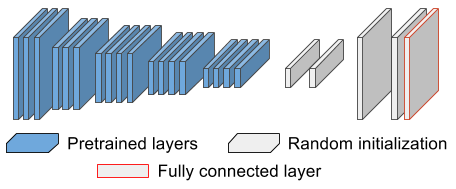
\includegraphics[width=0.8\linewidth,center]{images/part2/finetuning.png}
  \caption{Finetuning process}\textbf{
  \label{fig:part2:finetuning}}
\end{figure}

Actually, considering our small datasets, it is mandatory to use finetuning method for all of our experiments, a training from scratch would not be efficient. As an example, the curve~\ref{fig:part2:loss_bad} represents the loss function (function we try to minimize during the training, corresponding to a proportional inverse of the accuracy) we get while training from scratch. On the other hand, the curve~\ref{fig:part2:loss_good} is the one using finetuning.

\begin{figure}[ht!]
\centering
\begin{subfigure}{.5\textwidth}
  \centering
  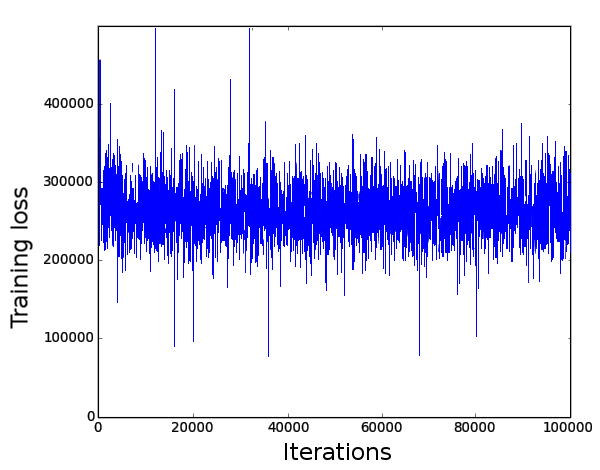
\includegraphics[width=0.9\linewidth]{images/part2/loss_bad.png}
  \caption{Loss without weight initialization}
  \label{fig:part2:loss_bad}
\end{subfigure}%
\begin{subfigure}{.5\textwidth}
  \centering
  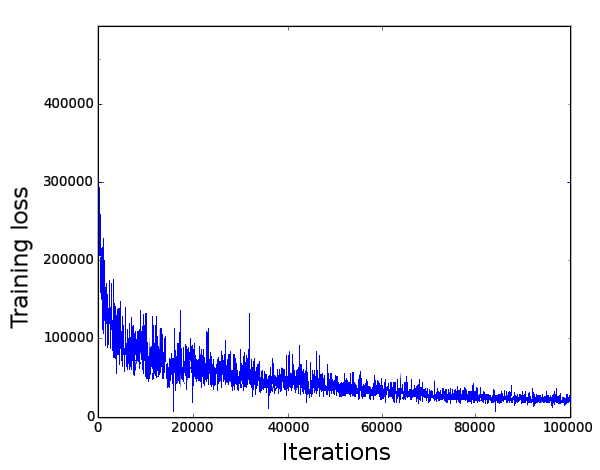
\includegraphics[width=0.9\linewidth]{images/part2/loss_good.png}
  \caption{Loss with weight initialization}
  \label{fig:part2:loss_good}
\end{subfigure}
\caption{Comparison of losses with or without initializations}
\label{fig:loss_comparison}
\end{figure}


\subsubsection{Multi-Source}
The multi-source transfer learning method~\cite{KAND16} can be more efficient, considering our project. Indeed, it has, as goal, to improve the general accuracy performed by one architecture on two different datasets. The main idea is to learn weights from the source dataset, then to finetune them with the target dataset, and to repeat these two operations for few cycles. Doing this, the learning of the source dataset is preserved, but also includes the features from the target dataset. This method improves the global accuracy (average of accuracies over both datasets), and also may improve the accuracy of the source dataset if it has some features close to the target. In our case, we have two datasets with aerial views, so the features from one dataset may help the architecture on the other one. This method can also be extended on more than two datasets, and also can be improved by playing on some parameters (such as decreasing the learning rate through the cycle). The figure~\ref{fig:part2:multisource} displays the functioning of Multi-Source over two dataset.

\todo{to clarify}
\begin{figure}[ht!]
  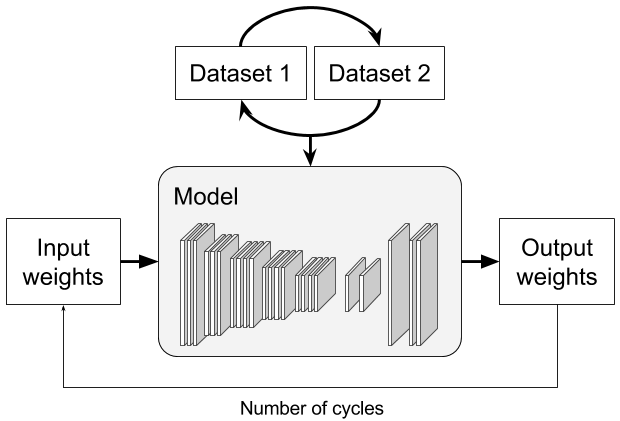
\includegraphics[width=0.8\linewidth,center]{images/part2/multisource.png}
  \caption{Multisource process between two datasets}\textbf{
  \label{fig:part2:multisource}}
\end{figure}





